%% 
%% Copyright 2019-2024 Elsevier Ltd
%% 
%% This file is part of the 'CAS Bundle'.
%% --------------------------------------
%% 
%% It may be distributed under the conditions of the LaTeX Project Public
%% License, either version 1.3c of this license or (at your option) any
%% later version.  The latest version of this license is in
%%    http://www.latex-project.org/lppl.txt
%% and version 1.3c or later is part of all distributions of LaTeX
%% version 1999/12/01 or later.
%% 
%% The list of all files belonging to the 'CAS Bundle' is
%% given in the file `manifest.txt'.
%% 
%% Template article for cas-dc documentclass for 
%% double column output.

\documentclass[a4paper,fleqn]{cas-dc}

% If the frontmatter runs over more than one page
% use the longmktitle option.

%\documentclass[a4paper,fleqn,longmktitle]{cas-dc}

%\usepackage[numbers]{natbib}
%\usepackage[authoryear]{natbib}
\usepackage[authoryear,longnamesfirst]{natbib}
\usepackage{tikz}
\usepackage{placeins}  % FloatBarrier support
% Insert float barrier at subsection boundaries
\let\origsubsection\subsection
\renewcommand{\subsection}{\FloatBarrier\origsubsection}

%%%Author macros
\def\tsc#1{\csdef{#1}{\textsc{\lowercase{#1}}\xspace}}
\tsc{WGM}
\tsc{QE}
%%%

% Uncomment and use as if needed
%\newtheorem{theorem}{Theorem}
%\newtheorem{lemma}[theorem]{Lemma}
%\newdefinition{rmk}{Remark}
%\newproof{pf}{Proof}
%\newproof{pot}{Proof of Theorem \ref{thm}}

\begin{document}
\let\WriteBookmarks\relax
\def\floatpagepagefraction{1}
\def\textpagefraction{.001}

% Relax float placement constraints
\renewcommand{\topfraction}{0.9}
\renewcommand{\bottomfraction}{0.9}
\renewcommand{\dbltopfraction}{0.9}
\renewcommand{\textfraction}{0.1}
\renewcommand{\floatpagefraction}{0.8}
\renewcommand{\dblfloatpagefraction}{0.8}

% Short title
\shorttitle{Thrust Profile Classification in LEO Transfers}

% Short author
\shortauthors{S. Lee}

% Main title of the paper
\title [mode = title]{Classification of Optimal Continuous Thrust Profiles for Low Earth Orbit Transfer Missions: A Parametric Database Study}

% Title footnote mark
% eg: \tnotemark[1]
%\tnotemark[1]

% Title footnote 1.
% eg: \tnotetext[1]{Title footnote text}
%\tnotetext[1]{} 

% First author
\author[1]{Suwon Lee}[orcid=0000-0002-6573-6348]

% Corresponding author indication
\cormark[1]

% Email id of the first author
\ead{suwon.lee@kookmin.ac.kr}

% Credit authorship
\credit{Conceptualization, Methodology, Software, Investigation, Writing - Original Draft}

% Address/affiliation
\affiliation[1]{organization={Department of Future Mobility, Kookmin University},
            addressline={77 Jeongneung-ro, Seongbuk-gu},
            city={Seoul},
            postcode={02707},
            country={Republic of Korea}}

% Corresponding author text
\cortext[1]{Corresponding author}

% Here goes the abstract
\begin{abstract}
This study presents a comprehensive parametric analysis of optimal continuous thrust profiles for low Earth orbit (LEO) transfer missions, motivated by the trajectory design needs of reusable space vehicles (ReUSVs) and LEO constellation operations. Using a two-pass direct collocation method, we generate a database of optimal trajectories across a five-dimensional configuration space encompassing semi-major axis change, inclination change, departure and arrival eccentricities, and transfer duration---the latter treated as a free optimization variable restricted to sub-single-revolution transfers. The resulting thrust profiles are systematically classified into unimodal (single-peak), bimodal (dual-peak), and multimodal (three or more peaks) types. Through automatic relevance determination (ARD) analysis, we identify the dominant configuration parameters governing thrust profile morphology. Furthermore, we establish a quantitative relationship between classical impulsive maneuvers and their continuous thrust counterparts, demonstrating that impulsive solutions represent limiting cases of the more general continuous optimal solutions. The results provide mission designers with predictive guidelines for anticipating optimal thrust profile characteristics based on transfer geometry, including transfers involving eccentric orbits.
\end{abstract}

% Use if graphical abstract is present
%\begin{graphicalabstract}
%\includegraphics{}
%\end{graphicalabstract}

% Research highlights
\begin{highlights}
\item Parametric database of optimal continuous thrust profiles for LEO transfers including eccentric orbits
\item Transfer duration as free optimization variable within sub-single-revolution bounds
\item Classification of thrust profiles into unimodal, bimodal, and multimodal types
\item Five-dimensional ARD analysis identifying dominant parameters governing profile morphology
\end{highlights}

% Keywords
% Each keyword is seperated by \sep
\begin{keywords}
Low-thrust trajectory optimization \sep Continuous thrust profile \sep Low Earth orbit transfer \sep Direct collocation \sep Parametric study
\end{keywords}

\maketitle

% Main text

%%%%%%%%%%%%%%%%%%%%%%%%%%%%%%%%%%%%%%%%%%%%%%%%%%%%%%%%%%%%%%%%%%
\section{Introduction}\label{sec:introduction}
%%%%%%%%%%%%%%%%%%%%%%%%%%%%%%%%%%%%%%%%%%%%%%%%%%%%%%%%%%%%%%%%%%

% Paragraph 1: ReUSV motivation and importance of continuous thrust
The growing interest in reusable space vehicles (ReUSVs) has introduced new demands on low Earth orbit (LEO) trajectory design \citep{Baiocco2021,Grantz2011}. After atmospheric reentry, a ReUSV must execute rapid orbit-raising maneuvers to return to its operational altitude; conversely, mission completion or rendezvous with a service platform may require controlled orbit-lowering transfers \citep{Jung2025}. These short-duration, sub-single-revolution maneuvers differ fundamentally from the multi-revolution spirals typical of electric propulsion (EP) station-keeping, yet they benefit from continuous thrust optimization to minimize propellant consumption and thermal loads during the transfer. Concurrently, the proliferation of LEO satellite constellations and the widespread adoption of EP systems \citep{Lev2019} have established continuous thrust trajectory optimization as an essential capability for modern space operations. EP systems such as ion thrusters and Hall-effect thrusters provide specific impulse ($I_{sp}$) values exceeding 2,000~seconds at the cost of lower thrust levels \citep{Jahn1968,Goebel2008}, and have been successfully deployed in missions including Dawn \citep{Rayman2000}, Hayabusa2 \citep{Tsuda2020}, SMART-1 \citep{Racca2002}, and the Starlink constellation \citep{SpaceNews2023}. The LEO environment presents unique challenges due to dominant $J_2$ perturbations from Earth's oblateness, frequent eclipse periods \citep{Graham2016}, and diverse transfer geometries involving both circular and elliptical orbits \citep{Topputo2014}.

% Paragraph 2: Overview of existing optimization methodologies
Extensive research has been devoted to developing efficient methods for low-thrust trajectory optimization \citep{Betts1998,Conway2010}. Direct methods transform the continuous optimal control problem into a finite-dimensional nonlinear programming (NLP) problem through discretization techniques such as Hermite-Simpson collocation \citep{Herman1996,Hargraves1987} and pseudospectral methods using Legendre-Gauss-Lobatto nodes \citep{Rao2025,Fahroo2002}. These approaches offer robust constraint handling and reliable convergence properties, with adaptive mesh refinement techniques further improving computational efficiency \citep{Patterson2014}. Convex optimization techniques, particularly successive convex programming (SCP) with lossless convexification \citep{Acikmese2013,Blackmore2012}, have emerged as powerful alternatives that guarantee polynomial-time complexity and avoid local minima traps inherent in nonlinear solvers \citep{Mao2017,Malyuta2022}. Indirect methods based on Pontryagin's minimum principle \citep{Pontryagin1962} provide theoretically optimal solutions but suffer from sensitivity to initial costate estimates, which has motivated the development of homotopy and continuation techniques \citep{Bertrand2002,Caillau2012}. More recently, machine learning approaches have been explored for costate initialization and thrust switching structure prediction \citep{Izzo2019,Zaidi2023}. Shape-based methods offer yet another paradigm, parameterizing trajectories using analytical basis functions such as B\'{e}zier curves \citep{Lee2021bezier} or exponential sinusoids, which can be particularly effective for short-duration transfers \citep{Lee2025eucass}. Despite this methodological diversity, existing studies predominantly focus on solving the forward problem: determining the optimal trajectory for a given specific mission configuration.

% Paragraph 3: Research gap - lack of systematic classification
Despite this progress, the systematic understanding of how mission parameters influence optimal thrust profile characteristics remains limited. Optimal continuous thrust trajectories exhibit distinct morphological features: thrust magnitude profiles display varying numbers of peaks separated by coasting (zero-thrust) arcs. These features are intimately connected to classical impulsive maneuvers---bimodal profiles with two thrust peaks correspond to two-impulse transfers such as the Hohmann maneuver \citep{Hohmann1960}, while multimodal profiles correspond to multi-impulse strategies \citep{Edelbaum1967}. However, no systematic framework exists to predict \textit{a priori} what type of thrust profile will emerge for a given transfer configuration, particularly when transfers involve eccentric orbits and short transfer durations relevant to ReUSV missions. Mission designers lack quantitative guidelines for anticipating whether a specific LEO-to-LEO transfer will yield a unimodal, bimodal, or multimodal optimal profile, and which orbital parameters---including eccentricity---most strongly influence this outcome.

% Paragraph 4: Research objectives and approach
This study addresses this gap by constructing a comprehensive database of optimal continuous thrust trajectories for LEO-to-LEO transfers---including eccentric orbits---and performing systematic classification and analysis of the resulting thrust profiles. The transfer duration is treated as a free optimization variable within prescribed bounds, restricting attention to sub-single-revolution transfers relevant to ReUSV orbit recovery and rendezvous scenarios. The specific objectives are threefold: (1) generate optimal trajectory solutions across a five-dimensional configuration space $(\Delta a, \Delta i, e_0, e_f, T_f)$ using direct collocation methods, (2) classify the thrust profiles into distinct types based on peak characteristics (unimodal, bimodal, and multimodal), and (3) identify the dominant orbital parameters that govern thrust profile morphology through statistical analysis. By establishing quantitative relationships between transfer geometry and optimal thrust profile type, this work provides predictive capability that enables mission designers to anticipate the general characteristics of optimal solutions before detailed optimization is performed. Furthermore, the correspondence between continuous thrust profile types and classical impulsive maneuvers is quantitatively examined, reinforcing the theoretical connection between these two trajectory design paradigms.

% Paragraph 5: Paper organization
The remainder of this paper is organized as follows. Section~\ref{sec:problem} formulates the continuous thrust trajectory optimization problem, establishes the relationship with impulsive maneuvers, and defines the cost function. Section~\ref{sec:methodology} describes the direct collocation methodology, database construction strategy, and thrust profile classification criteria. Section~\ref{sec:results_database} presents the generated database and analyzes the distribution of thrust profile types. Section~\ref{sec:results_geometric} provides geometric analysis of temporal profile characteristics. Section~\ref{sec:discussion} discusses the physical interpretation of results and practical implications. Finally, Section~\ref{sec:conclusions} summarizes the key findings and suggests directions for future research.


%%%%%%%%%%%%%%%%%%%%%%%%%%%%%%%%%%%%%%%%%%%%%%%%%%%%%%%%%%%%%%%%%%
\section{Problem Formulation}\label{sec:problem}
%%%%%%%%%%%%%%%%%%%%%%%%%%%%%%%%%%%%%%%%%%%%%%%%%%%%%%%%%%%%%%%%%%

\subsection{Continuous Thrust Trajectory Optimization}\label{subsec:continuous_thrust}

The trajectory optimization problem for continuous thrust LEO-to-LEO transfers is formulated as an optimal control problem. The spacecraft state and dynamics are defined in the Earth-Centered Inertial (ECI) frame. The formulation treats the transfer duration as a free optimization variable and parameterizes boundary orbits by their classical orbital elements, enabling systematic database construction over diverse transfer geometries.

\subsubsection{Equations of Motion}

The spacecraft state vector $\mathbf{x} \in \mathbb{R}^6$ consists of the position $\mathbf{r} \in \mathbb{R}^3$ and velocity $\mathbf{v} \in \mathbb{R}^3$ in the ECI frame:
\begin{equation}
\mathbf{x} = \begin{bmatrix} \mathbf{r} \\ \mathbf{v} \end{bmatrix}
\end{equation}

The equations of motion are given by:
\begin{equation}\label{eq:eom}
\dot{\mathbf{x}} = \begin{bmatrix} \dot{\mathbf{r}} \\ \dot{\mathbf{v}} \end{bmatrix} = \begin{bmatrix} \mathbf{v} \\ \mathbf{a}_{\text{grav}} + \mathbf{a}_{J_2} + \mathbf{a}_{\text{drag}} + \mathbf{a}_{\text{other}} + \mathbf{u} \end{bmatrix}
\end{equation}
where $\mathbf{u} \in \mathbb{R}^3$ is the thrust acceleration (control input), and the acceleration terms are defined as follows.

The two-body gravitational acceleration is:
\begin{equation}
\mathbf{a}_{\text{grav}} = -\frac{\mu}{r^3}\mathbf{r}
\end{equation}
where $\mu$ is the Earth's gravitational parameter and $r = \|\mathbf{r}\|$.

The $J_2$ perturbation acceleration, accounting for Earth's oblateness, is:
\begin{equation}
\mathbf{a}_{J_2} = -\frac{3\mu J_2 R_E^2}{2r^5} \begin{bmatrix}
x\left(1 - \frac{5z^2}{r^2}\right) \\[4pt]
y\left(1 - \frac{5z^2}{r^2}\right) \\[4pt]
z\left(3 - \frac{5z^2}{r^2}\right)
\end{bmatrix}
\end{equation}
where $J_2$ is the second zonal harmonic coefficient, $R_E$ is Earth's equatorial radius, and $(x, y, z)$ are the ECI position components.

The atmospheric drag acceleration is modeled as:
\begin{equation}
\mathbf{a}_{\text{drag}} = -\frac{1}{2}\rho(h) \frac{C_D A}{m} v_{\text{rel}} \mathbf{v}_{\text{rel}}
\end{equation}
where $\rho(h)$ is the atmospheric density at altitude $h$, $C_D$ is the drag coefficient, $A$ is the cross-sectional area, $m$ is the spacecraft mass, and $\mathbf{v}_{\text{rel}}$ is the velocity relative to the rotating atmosphere.

The term $\mathbf{a}_{\text{other}}$ encompasses additional perturbations such as solar radiation pressure, third-body gravitational effects, and higher-order gravitational harmonics, which may be included depending on mission fidelity requirements.

\subsubsection{Control Input}

The thrust acceleration $\mathbf{u}(t)$ serves as the control input, representing the acceleration produced by the electric propulsion system. This formulation decouples the trajectory optimization from specific propulsion system parameters (thrust magnitude and mass flow rate), allowing the results to be applicable across different spacecraft configurations.

\subsubsection{Boundary Conditions}

The departure and arrival orbits are specified by their classical orbital elements:
\begin{align}
\boldsymbol{\alpha}_0 &= (a_0, e_0, i_0, \Omega_0, \omega_0) \quad \text{(departure orbit)} \\
\boldsymbol{\alpha}_f &= (a_f, e_f, i_f, \Omega_f, \omega_f) \quad \text{(arrival orbit)}
\end{align}
where $a$ is the semi-major axis, $e$ is the eccentricity, $i$ is the inclination, $\Omega$ is the right ascension of the ascending node, and $\omega$ is the argument of periapsis.

The positions along the departure and arrival orbits, characterized by the true anomalies $\nu_0$ and $\nu_f$, are treated as free optimization variables. This formulation allows the optimizer to determine the optimal departure and arrival points on their respective orbits:
\begin{align}
\mathbf{x}(0) &= \mathbf{x}(\boldsymbol{\alpha}_0, \nu_0) \\
\mathbf{x}(T_f) &= \mathbf{x}(\boldsymbol{\alpha}_f, \nu_f)
\end{align}
where $T_f$ denotes the transfer duration. Unlike conventional formulations that fix $T_f$ as a specified parameter, this study treats $T_f$ as a free optimization variable subject to bound constraints:
\begin{equation}\label{eq:tf_bounds}
T_{\min} \leq T_f \leq T_{\max}
\end{equation}
This allows the optimizer to determine the energetically optimal transfer duration within a prescribed range. The bounds $T_{\min}$ and $T_{\max}$ are expressed in units of the initial orbital period $T_0 = 2\pi\sqrt{a_0^3/\mu}$ and are chosen to restrict attention to sub-single-revolution transfers (Section~\ref{subsec:configuration}).

\subsubsection{Constraints}

The optimization problem is subject to the following path constraints:

\textit{Thrust magnitude constraint:} The thrust acceleration is bounded above:
\begin{equation}
\|\mathbf{u}(t)\| \leq u_{\max}, \quad \forall t \in [0, T_f]
\end{equation}
Here $u_{\max}$ serves as a numerical safeguard rather than a physical propulsion limit. It is set sufficiently large (e.g., $u_{\max} = 1.0$~km/s$^2$) so that the bound is rarely active in practice; its purpose is to prevent the NLP solver from exploring physically unrealistic acceleration magnitudes during intermediate iterations.

\textit{Minimum altitude constraint:} To prevent atmospheric entry and ensure mission safety, the spacecraft altitude must remain above a specified minimum:
\begin{equation}
\|\mathbf{r}(t)\| \geq R_E + h_{\min}, \quad \forall t \in [0, T_f]
\end{equation}
where $h_{\min}$ is the minimum allowable altitude.

\subsubsection{Cost Function}

The cost function quantifies the control effort required for the orbital transfer. We adopt the energy-based (quadratic) cost function:
\begin{equation}\label{eq:cost_function}
J[\mathbf{u}(\cdot)] = \int_0^{T_f} \|\mathbf{u}(t)\|^2 \, dt
\end{equation}
which represents the integral of squared thrust acceleration over the transfer duration $T_f$.

The choice of $L^2$ norm over the $L^1$ norm (fuel-optimal formulation $\int \|\mathbf{u}\| dt$) is motivated by several considerations. The $L^1$ norm typically induces bang-bang control structures with discontinuous switching between maximum thrust and coasting, closely resembling impulsive maneuvers. In contrast, the $L^2$ norm yields smoother thrust profiles that are continuously differentiable, facilitating numerical optimization via direct collocation methods. Importantly, the $L^2$ formulation preserves the essential peak structure characteristics---the number and relative timing of thrust concentration regions---while avoiding the numerical challenges associated with detecting precise switching times. This makes it well-suited for the classification objectives of this study, where identifying the morphological type of thrust profiles is of primary interest rather than achieving minimum-fuel solutions.

\subsubsection{Optimal Control Problem Statement}

For a given orbital configuration $(\boldsymbol{\alpha}_0, \boldsymbol{\alpha}_f)$ and transfer duration bounds $[T_{\min}, T_{\max}]$, the continuous thrust trajectory optimization problem can be stated as:
\begin{equation}\label{eq:ocp}
\begin{aligned}
& \underset{\mathbf{u}(\cdot),\, \nu_0,\, \nu_f,\, T_f}{\text{minimize}} & & J[\mathbf{u}(\cdot)] \\
& \text{subject to} & & \dot{\mathbf{x}} = \mathbf{f}(\mathbf{x}, \mathbf{u}, t) \\
& & & \mathbf{x}(0) = \mathbf{x}(\boldsymbol{\alpha}_0, \nu_0) \\
& & & \mathbf{x}(T_f) = \mathbf{x}(\boldsymbol{\alpha}_f, \nu_f) \\
& & & T_{\min} \leq T_f \leq T_{\max} \\
& & & \|\mathbf{u}(t)\| \leq u_{\max}, \quad \forall t \in [0, T_f] \\
& & & \|\mathbf{r}(t)\| \geq R_E + h_{\min}, \quad \forall t \in [0, T_f]
\end{aligned}
\end{equation}
where $J$ is the cost function defined in Eq.~\eqref{eq:cost_function}, and $\mathbf{f}$ represents the right-hand side of Eq.~\eqref{eq:eom}. The decision variables include the thrust acceleration profile $\mathbf{u}(t)$, the departure/arrival true anomalies $\nu_0$ and $\nu_f$, and the transfer duration $T_f$.

This formulation enables systematic parametric studies by varying the orbital configuration---defined by the differences in orbital elements $(\Delta a, \Delta i, e_0, e_f)$ between the departure and arrival orbits---while letting the optimizer determine the energetically optimal transfer duration within the prescribed bounds.

\subsection{Relationship with Impulsive Maneuvers}\label{subsec:impulsive_relation}

The continuous thrust formulation presented in Section~\ref{subsec:continuous_thrust} encompasses impulsive maneuvers as a limiting case. This relationship provides both theoretical justification for our approach and practical insight into interpreting continuous thrust profiles.

\subsubsection{Mathematical Representation of Impulsive Maneuvers}

An impulsive maneuver is characterized by an instantaneous velocity change $\Delta\mathbf{v}$ at time $t_k$, which can be mathematically represented using the Dirac delta function \citep{Lawden1963}:
\begin{equation}\label{eq:impulse_delta}
\mathbf{u}_{\text{imp}}(t) = \Delta\mathbf{v}_k \cdot \delta(t - t_k)
\end{equation}
where $\delta(\cdot)$ denotes the Dirac delta function. For an $N$-impulse trajectory, the control input becomes:
\begin{equation}\label{eq:n_impulse}
\mathbf{u}_{\text{imp}}(t) = \sum_{k=1}^{N} \Delta\mathbf{v}_k \cdot \delta(t - t_k)
\end{equation}

This representation reveals that impulsive maneuvers constitute a special case of the general continuous thrust formulation, where the control is concentrated at discrete time instants with infinite magnitude but finite integral (velocity change).

\subsubsection{Solution Space Inclusion}

A fundamental relationship exists between the solution spaces of continuous and impulsive trajectory optimization problems. Let $\mathcal{S}_{\text{cont}}$ denote the set of feasible trajectories under continuous thrust control and $\mathcal{S}_{\text{imp}}$ denote the set of feasible trajectories under $N$-impulse control. The following inclusion relationship holds \citep{Taheri2020}:
\begin{equation}\label{eq:solution_space}
\mathcal{S}_{\text{imp}} \subset \mathcal{S}_{\text{cont}}
\end{equation}

This relationship implies that any trajectory achievable through impulsive maneuvers can also be achieved (or closely approximated) by continuous thrust, but not vice versa. Consequently, the optimal cost for continuous thrust problems is bounded above by the optimal impulsive solution:
\begin{equation}
J^*_{\text{cont}} \leq J^*_{\text{imp}}
\end{equation}

Furthermore, as the number of impulses $N$ increases, the impulsive solution converges to the continuous optimal solution under appropriate regularity conditions \citep{Prussing2010}.

\subsubsection{Correspondence Between Thrust Profiles and Classical Maneuvers}

The solution space relationship suggests a correspondence between continuous thrust profile characteristics and classical impulsive maneuvers:

\begin{itemize}
\item \textit{Unimodal profiles} (single thrust peak) correspond to single-impulse maneuvers, typically observed in transfers requiring primarily velocity magnitude changes at a single orbital location.

\item \textit{Bimodal profiles} (dual thrust peaks) correspond to two-impulse maneuvers such as the Hohmann transfer, where thrust concentration occurs at the departure and arrival regions.

\item \textit{Multimodal profiles} (three or more peaks) correspond to multi-impulse maneuvers such as bi-elliptic transfers, which become optimal for large orbital ratio changes.
\end{itemize}

This correspondence provides physical intuition for interpreting the thrust profile classification results presented in this study. The continuous optimal solution ``smooths'' the impulsive solution while preserving its fundamental structure, with thrust peaks occurring at locations analogous to impulsive burn points.


%%%%%%%%%%%%%%%%%%%%%%%%%%%%%%%%%%%%%%%%%%%%%%%%%%%%%%%%%%%%%%%%%%
\section{Methodology}\label{sec:methodology}
%%%%%%%%%%%%%%%%%%%%%%%%%%%%%%%%%%%%%%%%%%%%%%%%%%%%%%%%%%%%%%%%%%

\subsection{Two-Pass Direct Collocation Method}\label{subsec:direct_collocation}

The continuous optimal control problem defined in Eq.~\eqref{eq:ocp} is transcribed into a finite-dimensional nonlinear programming (NLP) problem using a two-pass direct collocation approach. This hybrid method combines the uniform sampling advantages of Hermite-Simpson collocation with the high accuracy of Legendre-Gauss-Lobatto (LGL) pseudospectral methods \citep{Hargraves1987,Rao2025,Fahroo2002}.

The motivation for this two-pass approach stems from a fundamental challenge in pseudospectral methods: LGL nodes are clustered near the domain boundaries, which may not align with the thrust concentration regions (peaks) in the optimal solution. Since peak locations are unknown \textit{a priori}, a preliminary optimization with uniformly distributed nodes is first performed to identify the thrust profile structure, followed by a refined optimization with adaptive node placement.

\subsubsection{Pass 1: Hermite-Simpson Collocation}

The first pass employs Hermite-Simpson collocation with uniformly spaced nodes to obtain a preliminary solution and identify thrust peak locations. The transfer duration $[0, T_f]$ is divided into $M$ equal segments of width $h = T_f/M$. Within each segment $[t_k, t_{k+1}]$, the state trajectory is approximated by a cubic Hermite polynomial, with collocation enforced at the segment midpoint using Simpson's rule.

The collocation constraints for each segment are:
\begin{align}
\mathbf{x}_{k+1} &= \mathbf{x}_k + \frac{h}{6}\left[\mathbf{f}_k + 4\mathbf{f}_{k+\frac{1}{2}} + \mathbf{f}_{k+1}\right] \label{eq:simpson_continuity} \\
\mathbf{x}_{k+\frac{1}{2}} &= \frac{1}{2}(\mathbf{x}_k + \mathbf{x}_{k+1}) + \frac{h}{8}(\mathbf{f}_k - \mathbf{f}_{k+1}) \label{eq:hermite_midpoint}
\end{align}
where $\mathbf{f}_k = \mathbf{f}(\mathbf{x}_k, \mathbf{u}_k)$ denotes the dynamics evaluated at node $k$. The cost function is approximated using Simpson's quadrature:
\begin{equation}
J \approx \sum_{k=0}^{M-1} \frac{h}{6}\left[\|\mathbf{u}_k\|^2 + 4\|\mathbf{u}_{k+\frac{1}{2}}\|^2 + \|\mathbf{u}_{k+1}\|^2\right]
\end{equation}

For the database construction, $M = 30$ segments are used, yielding 61 collocation points (31 primary nodes plus 30 midpoints) and approximately 550 decision variables. The uniform node distribution ensures that thrust peaks are captured regardless of their temporal location.

\subsubsection{Peak Detection}

Upon convergence of Pass 1, the thrust magnitude profile $\|\mathbf{u}(t)\|$ is analyzed to identify local maxima corresponding to thrust concentration regions. Peaks are detected using a topological persistence algorithm based on 0-dimensional persistent homology (Section~\ref{subsec:classification}). The number of detected peaks determines the thrust profile classification (unimodal, bimodal, or multimodal) and informs the phase structure for Pass 2.

\subsubsection{Pass 2: Multi-Phase LGL Collocation}

The second pass employs a multi-phase formulation where the transfer is partitioned into distinct phases based on the detected peak structure. Each phase is discretized independently using LGL nodes, with higher node density allocated to peak regions and lower density to coasting regions.

For a problem with $n_p$ detected peaks, the transfer is divided into $2n_p - 1$ phases: $n_p$ peak phases centered on the detected peak times and $n_p - 1$ coasting phases in between. The phase boundaries are included as optimization variables, allowing the solver to refine the peak locations.

Within each phase $p$ spanning $[T_{p-1}, T_p]$, the time coordinate is transformed to $\sigma \in [-1, 1]$:
\begin{equation}
t = T_{p-1} + \frac{T_p - T_{p-1}}{2}(\sigma + 1)
\end{equation}

The state and control within phase $p$ are approximated at $N_p + 1$ LGL nodes. The state trajectory is represented by Lagrange interpolating polynomials:
\begin{equation}
\mathbf{x}^{(p)}(\sigma) \approx \sum_{j=0}^{N_p} \mathbf{x}_j^{(p)} L_j(\sigma)
\end{equation}
and the dynamics constraints are enforced as:
\begin{equation}
\frac{2}{T_p - T_{p-1}} \sum_{j=0}^{N_p} D_{ij}^{(p)} \mathbf{x}_j^{(p)} = \mathbf{f}(\mathbf{x}_i^{(p)}, \mathbf{u}_i^{(p)})
\end{equation}
where $\mathbf{D}^{(p)}$ is the LGL differentiation matrix for phase $p$.

Continuity across phase boundaries is enforced through linkage constraints:
\begin{equation}
\mathbf{x}^{(p)}(\sigma = 1) = \mathbf{x}^{(p+1)}(\sigma = -1), \quad p = 1, \ldots, P-1
\end{equation}

The cost function is the sum of contributions from all phases:
\begin{equation}
J \approx \sum_{p=1}^{P} \frac{T_p - T_{p-1}}{2} \sum_{j=0}^{N_p} w_j^{(p)} \|\mathbf{u}_j^{(p)}\|^2
\end{equation}
where $w_j^{(p)}$ are the LGL quadrature weights for phase $p$.

For the database construction, peak phases are discretized with $N_{\text{peak}} = 15$ nodes and coasting phases with $N_{\text{coast}} = 8$ nodes. The solution from Pass 1 is interpolated onto the LGL nodes to provide a warm-start initial guess, significantly improving convergence reliability.

\subsubsection{Implementation}

Both optimization passes are formulated using the CasADi symbolic framework \citep{Andersson2019} with the Opti stack interface, and solved by the interior-point solver IPOPT \citep{Waechter2006} with the MUMPS linear solver. CasADi provides automatic differentiation of cost and constraint functions, supplying exact Jacobians and Hessians to IPOPT without manual derivation. Pass~1 uses relaxed convergence tolerances ($10^{-4}$) for rapid preliminary solution, while Pass~2 employs tighter tolerances ($10^{-6}$) for the final high-accuracy solution. The Pass~1 solution is interpolated onto the LGL nodes to warm-start Pass~2.

The two-pass approach typically requires less than 3~seconds per case on a modern workstation, enabling systematic generation of large trajectory databases.

\subsection{Configuration Space and Sampling}\label{subsec:configuration}

To systematically investigate how orbital transfer geometry influences optimal thrust profile characteristics, a parametric study is conducted over a carefully defined configuration space. The configuration parameters, their ranges, and the sampling strategy are described below.

\subsubsection{Configuration Parameters}

The configuration space is defined by five primary parameters that characterize the orbital transfer geometry:

\begin{itemize}
\item \textit{Semi-major axis change} ($\Delta a = a_f - a_0$): The difference in semi-major axis between the arrival and departure orbits. This parameter governs the energy requirement of the transfer and encompasses both orbit-raising (e.g., post-reentry altitude recovery) and orbit-lowering (e.g., controlled deorbit) scenarios relevant to reusable space vehicle (ReUSV) missions.

\item \textit{Inclination change} ($\Delta i = i_f - i_0$): The change in orbital plane inclination. Plane changes are among the most costly maneuvers in orbital mechanics, requiring velocity changes perpendicular to the orbital plane.

\item \textit{Departure eccentricity} ($e_0$): The eccentricity of the departure orbit. Including $e_0$ as an independent parameter accommodates transfers originating from elliptical parking orbits, which arise naturally in ReUSV missions after atmospheric skip or aerocapture maneuvers.

\item \textit{Arrival eccentricity} ($e_f$): The eccentricity of the target orbit. Treating $e_f$ independently from $e_0$ enables the study of circularization maneuvers ($e_0 > 0, e_f = 0$) as well as transfers to elliptical target orbits.

\item \textit{Transfer duration bounds} ($[T_{\min}, T_{\max}]$): The allowable range for the free transfer duration $T_f$, expressed in units of the initial orbital period $T_0 = 2\pi\sqrt{a_0^3/\mu}$. This study restricts attention to short-duration transfers with $T_f/T_0 \leq 1.2$, corresponding to sub-single-revolution maneuvers that are characteristic of high-thrust-like continuous thrust operations.
\end{itemize}

Additionally, the initial orbit altitude ($h_0 = a_0 - R_E$) serves as a secondary parameter for slice-wise analysis, enabling investigation of how the classification boundaries shift with orbital altitude.

The right ascension of the ascending node is held constant ($\Omega_0 = \Omega_f = 0$). Under the two-body gravitational field with $J_2$ zonal harmonics---which preserves rotational symmetry about the Earth's polar axis---the absolute value of $\Omega$ does not affect the trajectory optimization; this reduction is valid without loss of generality \citep{Vallado2013}. The argument of periapsis is also held constant ($\omega_0 = \omega_f = 0$). For circular orbits ($e = 0$), $\omega$ is undefined, making this choice trivially valid. For elliptical orbits ($e > 0$), fixing $\omega$ restricts the apse line orientation; the influence of $\omega$ as an independent parameter is deferred to future work \citep{Curtis2020}.

\subsubsection{Parameter Ranges}

The parameter ranges are selected to cover operationally relevant LEO transfer scenarios:

\begin{table}[ht]
\centering
\caption{Configuration parameter ranges for the parametric study.}
\label{tab:param_ranges}
\begin{tabular}{lccc}
\hline
Parameter & Symbol & Range & Unit \\
\hline
Semi-major axis change & $\Delta a$ & $[-500,\; 2000]$ & km \\
Inclination change & $\Delta i$ & $[0,\; 15]$ & deg \\
Departure eccentricity & $e_0$ & $[0,\; 0.1]$ & -- \\
Arrival eccentricity & $e_f$ & $[0,\; 0.1]$ & -- \\
Transfer duration bounds & $T_f/T_0$ & $[0.1,\; 1.2]$ & -- \\
Initial altitude & $h_0$ & $\{400, 600, 800, 1000\}$ & km \\
\hline
\end{tabular}
\end{table}

The semi-major axis range encompasses both orbit-lowering maneuvers (negative $\Delta a$, relevant for ReUSV controlled deorbit or collision avoidance) and orbit-raising maneuvers (positive $\Delta a$, relevant for post-reentry orbit recovery or constellation deployment). The inclination change range covers practical plane change requirements for ground track optimization and mission phasing. The eccentricity parameters $e_0$ and $e_f$ are treated independently, enabling the study of diverse transfer geometries: circular-to-circular ($e_0 = e_f = 0$), elliptical-to-circular (circularization), circular-to-elliptical, and elliptical-to-elliptical transfers. The transfer duration upper bound $T_f/T_0 \leq 1.2$ restricts the database to sub-single-revolution transfers, which are characteristic of short-duration maneuvers relevant to ReUSV orbit recovery and rendezvous scenarios where rapid orbit adjustment is required.

\subsubsection{Adaptive Sampling Strategy}

Rather than employing uniform grid sampling, which would require prohibitively many samples to adequately resolve classification boundaries, an adaptive sampling strategy is adopted. The approach consists of two phases:

\textit{Phase 1: Initial coverage sampling.} Latin Hypercube Sampling (LHS) is used to generate an initial set of $N_{\text{init}}$ samples distributed throughout the five-dimensional parameter space $(\Delta a, \Delta i, e_0, e_f, T_{\max}/T_0)$. This space-filling design ensures adequate coverage of the configuration space while avoiding clustering.

\textit{Phase 2: Boundary-focused adaptive sampling.} A Gaussian Process (GP) classifier is trained on the initial samples, providing probabilistic predictions of thrust profile class membership across the parameter space. New samples are iteratively selected at locations where the classification uncertainty is highest, effectively concentrating sampling effort near the boundaries between different thrust profile regimes. This approach is based on active learning principles \citep{Settles2009} and has been successfully applied to classification boundary identification in dynamical systems \citep{Lee2023}. The entropy-based acquisition function admits an information-theoretic interpretation: sampling at high-entropy locations maximally reduces uncertainty about the classification boundaries, achieving near-optimal sample complexity that scales with boundary complexity rather than parameter space volume. The mathematical details of the GP-based sampling procedure are provided in Appendix~\ref{app:gp_sampling}.

The adaptive sampling continues until either a maximum of $N_{\text{max}} = 800$ samples is reached or the maximum predictive entropy falls below a convergence threshold of 0.3. For each altitude slice, 150 initial LHS samples are generated, followed by iterative batches of 15 actively selected samples. In practice, all four altitude slices reached the maximum sample count of 810 (150 initial + 44 batches $\times$ 15).

\subsection{Thrust Profile Classification}\label{subsec:classification}

The classification of optimal thrust profiles is based on the number and characteristics of thrust magnitude peaks identified in the converged solution from Pass~1 of the two-pass optimization (Section~\ref{subsec:direct_collocation}).

\subsubsection{Classification Criteria}

Three distinct classes are defined based on peak count:

\begin{itemize}
\item \textit{Unimodal} (Class 0): Single thrust peak. The thrust magnitude profile exhibits one dominant maximum, corresponding to concentrated propulsive effort at a single orbital location. This pattern is analogous to single-impulse maneuvers.

\item \textit{Bimodal} (Class 1): Two thrust peaks. The profile shows two distinct maxima separated by a low-thrust or coasting region. This pattern corresponds to classical two-impulse maneuvers such as the Hohmann transfer.

\item \textit{Multimodal} (Class 2): Three or more thrust peaks. The profile exhibits multiple distinct maxima, corresponding to multi-impulse strategies such as bi-elliptic transfers.
\end{itemize}

\subsubsection{Peak Detection Algorithm}

Peaks in the thrust magnitude profile $\|\mathbf{u}(t)\|$ are identified using a topological persistence algorithm based on 0-dimensional persistent homology \citep{Edelsbrunner2010,Huber2021}. This approach offers three advantages over conventional methods such as SciPy's \texttt{find\_peaks} with prominence filtering: (i)~it requires only a single threshold parameter, (ii)~it handles boundary peaks (at $t = 0$ or $t = T_f$) without additional logic, and (iii)~it is robust to interpolation artifacts from sparse collocation data.

The algorithm conceptually sweeps a horizontal threshold from the global maximum downward through the profile. When the threshold crosses a local maximum, a new connected component is born; when it crosses a local minimum between two components, the younger component (lower birth value) merges into the older one and dies. This merging rule is known as the \textit{Elder rule} \citep{Edelsbrunner2010}. The \textit{persistence} of each peak is the difference between its birth value (peak height) and death value (merging level):
\begin{equation}
  \mathrm{pers}(p) = f(b_p) - f(d_p)
  \label{eq:persistence}
\end{equation}
The global maximum has infinite persistence by convention. A peak is classified as significant if its persistence exceeds a fraction $\alpha$ of the global maximum thrust magnitude:
\begin{equation}
  \mathcal{S} = \bigl\{p \mid \mathrm{pers}(p) \geq \alpha \cdot \max_t \|\mathbf{u}(t)\| \bigr\}
  \label{eq:significant_peaks}
\end{equation}
with $\alpha = 0.10$ used throughout this study (Fig.~\ref{fig:peak_detection_schematic}).

Since the pseudospectral collocation solution is defined at only 15--30 non-uniform nodes, the thrust magnitude is first interpolated onto $N_{\mathrm{interp}} = 200$ uniformly spaced points using cubic splines before peak detection. For multi-phase solutions, interpolation is performed independently within each phase to avoid Runge-like oscillations at phase boundaries.

\begin{figure}[ht]
\centering
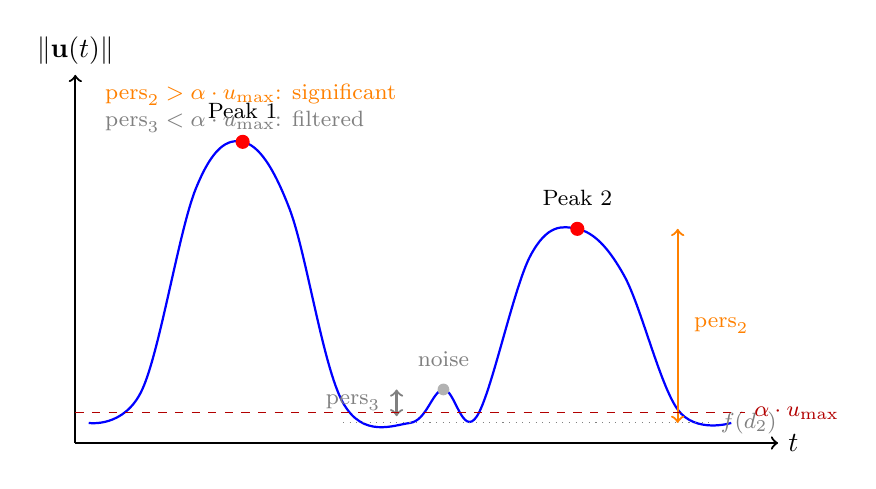
\begin{tikzpicture}[scale=0.85]
  % Axes
  \draw[->,thick] (0,0) -- (10.5,0) node[right] {$t$};
  \draw[->,thick] (0,0) -- (0,5.5) node[above] {$\|\mathbf{u}(t)\|$};
  % Thrust profile (bimodal with a noise bump)
  \draw[thick,blue] plot[smooth,tension=0.6] coordinates {
    (0.2,0.3) (1.0,0.8) (1.8,3.8) (2.5,4.5) (3.2,3.5) (4.0,0.6)
    (5.0,0.3) (5.5,0.8) (6.0,0.4) (6.8,2.8) (7.5,3.2) (8.2,2.5) (9.0,0.5) (9.8,0.3)
  };
  % Peak markers
  \fill[red] (2.5,4.5) circle (3pt);
  \fill[red] (7.5,3.2) circle (3pt);
  \fill[gray!60] (5.5,0.8) circle (2.5pt);
  \node[above] at (2.5,4.7) {\footnotesize Peak 1};
  \node[above] at (7.5,3.4) {\footnotesize Peak 2};
  \node[above,gray] at (5.5,1.0) {\footnotesize noise};
  % Death level for Peak 2 (local min between peaks)
  \draw[dotted,gray] (4.0,0.3) -- (9.5,0.3);
  \node[gray,right] at (9.5,0.3) {\footnotesize $f(d_2)$};
  % Persistence arrow for Peak 2
  \draw[<->,thick,orange] (9.0,0.3) -- (9.0,3.2);
  \node[orange,right] at (9.1,1.75) {\footnotesize $\mathrm{pers}_2$};
  % Persistence arrow for noise peak (small)
  \draw[<->,thick,gray] (4.8,0.4) -- (4.8,0.8);
  \node[gray,left] at (4.7,0.6) {\footnotesize $\mathrm{pers}_3$};
  % Threshold line
  \draw[dashed,red!70!black] (0,0.45) -- (10,0.45);
  \node[red!70!black,right] at (10,0.45) {\footnotesize $\alpha \cdot u_{\max}$};
  % Annotations
  \node[orange,anchor=west] at (0.3,5.2) {\footnotesize $\mathrm{pers}_2 > \alpha \cdot u_{\max}$: significant};
  \node[gray,anchor=west] at (0.3,4.8) {\footnotesize $\mathrm{pers}_3 < \alpha \cdot u_{\max}$: filtered};
\end{tikzpicture}
\caption{Schematic illustration of the persistence-based peak detection. Each peak's persistence measures the height difference between its birth (peak value) and death (merging level). Peak~2 survives the threshold $\alpha \cdot u_{\max}$ while the noise bump is filtered out. Peak~1 (global maximum) has infinite persistence.}
\label{fig:peak_detection_schematic}
\end{figure}

\subsubsection{Verification}

The topological persistence algorithm was validated on synthetic Gaussian profiles with 1, 2, and 3 known peaks, correctly identifying all peak counts and locations (position error $< 0.05\,T_f$). Edge cases---zero signal, constant signal, and boundary peaks at $t = 0$ or $t = T_f$---were all handled correctly without special-case logic. Noise robustness was confirmed by adding perturbations of $\sigma = 10^{-3}$ to synthetic profiles without affecting the classification outcome. The algorithm was also compared against three alternative methods---SciPy \texttt{find\_peaks} with prominence filtering, Savitzky--Golay zero-crossing, and continuous wavelet transform (CWT)---on eight test cases combining synthetic and actual LGL collocation solutions. The topological persistence method achieved the highest agreement (88\%) with the baseline while correctly resolving all disagreement cases upon visual inspection; CWT suffered from over-detection on sparse LGL data (7--9 spurious peaks), and Savitzky--Golay was sensitive to window size.


%%%%%%%%%%%%%%%%%%%%%%%%%%%%%%%%%%%%%%%%%%%%%%%%%%%%%%%%%%%%%%%%%%
\section{Results: Thrust Profile Database}\label{sec:results_database}
%%%%%%%%%%%%%%%%%%%%%%%%%%%%%%%%%%%%%%%%%%%%%%%%%%%%%%%%%%%%%%%%%%

\subsection{Overview of Database}\label{subsec:database_overview}

The adaptive sampling strategy described in Section~\ref{subsec:configuration} was applied independently to each of the four initial altitude slices ($h_0 = 400$, 600, 800, and 1000~km). Table~\ref{tab:db_summary} summarizes the resulting trajectory database.

\begin{table}[ht]
\centering
\caption{Summary of the trajectory database across the five-dimensional configuration space.}
\label{tab:db_summary}
\begin{tabular}{rrrrccc}
\hline
$h_0$ [km] & Total & Converged & Rate [\%] & Unimodal & Bimodal & Multimodal \\
\hline
400 & 810 & 331 & 40.9 & 25 & 219 & 87 \\
600 & 810 & 423 & 52.2 & 12 & 167 & 244 \\
800 & 810 & 289 & 35.7 & 12 & 217 & 60 \\
1000 & 810 & 720 & 88.9 & 23 & 405 & 292 \\
\hline
Total & 3240 & 1763 & 54.4 & 72 & 1008 & 683 \\
\hline
\end{tabular}
\end{table}

The overall convergence rate is 54.4\% (1763 of 3240 cases), with significant variation across altitude slices: $h_0 = 1000$~km achieves the highest rate (88.9\%), while $h_0 = 800$~km has the lowest (35.7\%). Non-convergence is strongly correlated with short transfer durations: cases with $T_{\max}/T_0 < 0.375$ converge at only 23.0\%, compared to 72--87\% for longer durations. This is expected because short-duration transfers impose tight constraints on the available thrust time relative to the required orbital element change. The current formulation with $T_f$ as a free variable attributes non-convergence primarily to cases where the prescribed duration range $[T_{\min}, T_{\max}]$ is insufficient to accomplish the required orbital change.

The adaptive sampling effectively concentrated samples near classification boundaries (Fig.~\ref{fig:sampling_progress}). All four altitude slices reached the maximum sample count before the entropy convergence threshold was met, indicating that the five-dimensional classification boundaries are sufficiently complex to warrant the full sampling budget.

\begin{figure}[ht]
\centering
\includegraphics[width=\columnwidth]{figures/fig7_sampling_progress.pdf}
\caption{Adaptive sampling convergence for each initial altitude slice, showing the cumulative number of evaluated samples.}
\label{fig:sampling_progress}
\end{figure}

\subsection{Thrust Profile Type Distribution}\label{subsec:type_distribution}

The three thrust profile types---unimodal, bimodal, and multimodal---are illustrated in Fig.~\ref{fig:representative_profiles} through representative examples selected from the database.

\begin{figure*}[!htbp]
\centering
\includegraphics[width=\textwidth]{figures/fig1_representative_profiles.pdf}
\caption{Representative thrust magnitude profiles for each classification type: (a)~unimodal with a single thrust peak, (b)~bimodal with two distinct thrust peaks separated by a coasting region, and (c)~multimodal with three or more peaks. The horizontal axis shows normalized mission time $t/T_f$ and the vertical axis shows thrust magnitude in $\times 10^{-3}$~km/s$^2$. Examples are selected from the median-cost case within each class, with physically validated trajectory data.}
\label{fig:representative_profiles}
\end{figure*}

The unimodal profile (Fig.~\ref{fig:representative_profiles}a) exhibits a single smooth thrust peak, concentrating propulsive effort at one orbital location. This pattern prevails in transfers with short durations, where the spacecraft has insufficient time for multiple thrust arcs.

The bimodal profile (Fig.~\ref{fig:representative_profiles}b) displays two distinct thrust peaks separated by a near-zero thrust coasting region. This structure directly corresponds to the classical two-impulse Hohmann transfer geometry, where thrust is concentrated at the departure and arrival orbital positions. Bimodal profiles constitute the majority of the database (57.2\% of converged cases), consistent with the prevalence of two-impulse-like solutions in sub-single-revolution transfers.

The multimodal profile (Fig.~\ref{fig:representative_profiles}c) exhibits three or more thrust peaks with intervening coasting arcs. Because the current database is restricted to sub-single-revolution transfers ($T_f/T_0 \leq 1.2$), multimodal profiles are expected to occur less frequently than in the multi-revolution regime, arising primarily in transfers with large combined altitude-inclination-eccentricity changes where multi-burn strategies remain energetically favorable even within a single orbital revolution.

\begin{figure*}[!htbp]
\centering
\includegraphics[width=\textwidth]{figures/fig2_representative_trajectories.pdf}
\caption{Three-dimensional ECI trajectories corresponding to the representative profiles in Fig.~\ref{fig:representative_profiles}: (a)~unimodal, (b)~bimodal, (c)~multimodal.}
\label{fig:representative_trajectories}
\end{figure*}

The corresponding 3D trajectories are shown in Fig.~\ref{fig:representative_trajectories}. The unimodal case (a) exhibits a nearly direct transfer arc, while the bimodal case (b) shows a transfer geometry resembling an elliptical Hohmann orbit. The multimodal case (c) displays a sub-single-revolution trajectory with multiple distinct thrust arcs at geometrically favorable orbital positions.

Table~\ref{tab:class_cost} summarizes the $L^2$ cost statistics for each profile class. The cost $J$ has units of km$^2$/s$^3$ (squared acceleration integrated over time). Dimensionally, for a transfer requiring a characteristic velocity change $\Delta v$ over duration $T_f$, the cost scales as $J \sim (\Delta v)^2 / T_f$, reflecting the trade-off between maneuver magnitude and available transfer time.

\begin{table}[ht]
\centering
\caption{$L^2$ cost statistics by profile class (converged cases only). The cost $J$ has units of km$^2$/s$^3$.}
\label{tab:class_cost}
\begin{tabular}{lrccc}
\hline
Class & Count & Mean $J$ & Std $J$ & Max $J$ \\
\hline
Unimodal & 72 & $1.47 \times 10^{-3}$ & $1.98 \times 10^{-3}$ & $1.59 \times 10^{-2}$ \\
Bimodal & 1008 & $6.19 \times 10^{-3}$ & $2.00 \times 10^{-2}$ & $2.89 \times 10^{-1}$ \\
Multimodal & 683 & $1.26 \times 10^{-2}$ & $5.40 \times 10^{-2}$ & $4.87 \times 10^{-1}$ \\
\hline
\end{tabular}
\end{table}

\subsection{Dominant Factor Analysis}\label{subsec:dominant_factors}

To identify which configuration parameters most strongly influence thrust profile classification, we examine the classification maps and ARD kernel length scales from the GP classifier.

\subsubsection{Classification Maps}

Figs.~\ref{fig:classification_da_di}--\ref{fig:classification_di_T} present 2D projections of the classification results for each altitude slice. Each point represents a converged trajectory colored by its profile class, projected onto the selected pair of configuration parameters. Because the remaining parameters ($e_0$, $e_f$, and/or $T_f/T_0$) vary across the projected points, these scatter plots display the marginal distribution of profile classes rather than a slice at fixed parameter values. This approach reveals the overall structure of the classification landscape without requiring parameter fixing.

\begin{figure*}[!htbp]
\centering
\includegraphics[width=\textwidth]{figures/fig3_classification_da_di.pdf}
\caption{Classification map in the $\Delta a$--$\Delta i$ plane for each initial altitude: (a)~$h_0 = 400$~km, (b)~$h_0 = 600$~km, (c)~$h_0 = 800$~km, (d)~$h_0 = 1000$~km.}
\label{fig:classification_da_di}
\end{figure*}

\begin{figure*}[!htbp]
\centering
\includegraphics[width=\textwidth]{figures/fig4_classification_da_T.pdf}
\caption{Classification map in the $\Delta a$--$T_f/T_0$ plane for each initial altitude.}
\label{fig:classification_da_T}
\end{figure*}

\begin{figure*}[!htbp]
\centering
\includegraphics[width=\textwidth]{figures/fig5_classification_di_T.pdf}
\caption{Classification map in the $\Delta i$--$T_f/T_0$ plane for each initial altitude.}
\label{fig:classification_di_T}
\end{figure*}

The $\Delta a$--$T_f/T_0$ (Fig.~\ref{fig:classification_da_T}) and $\Delta i$--$T_f/T_0$ (Fig.~\ref{fig:classification_di_T}) projections reveal the clearest separation between profile types, indicating that the transfer duration $T_f/T_0$ plays a dominant role in determining the thrust profile morphology. In contrast, the $\Delta a$--$\Delta i$ projection (Fig.~\ref{fig:classification_da_di}) shows more overlap between classes, suggesting that the orbital element changes alone are insufficient to predict the profile type. Projections onto the eccentricity dimensions are not shown because the ARD analysis (Section~\ref{subsec:dominant_factors}) indicates that $e_0$ and $e_f$ have weak to negligible influence on the classification.

A 3D visualization of the classification map (Fig.~\ref{fig:classification_3d}) confirms that the classification boundaries form surfaces in the parameter space, with $T_f/T_0$ providing the primary axis of separation.

\begin{figure}[ht]
\centering
\includegraphics[width=\columnwidth]{figures/fig6_classification_3d.pdf}
\caption{Three-dimensional classification map for $h_0 = 1000$~km (altitude slice with the most converged cases).}
\label{fig:classification_3d}
\end{figure}

\subsubsection{ARD Length Scale Analysis}

The ARD kernel length scales from the GP classifier quantify how sensitively the classification depends on each input parameter. A shorter length scale means the classification function varies more rapidly along that dimension, indicating stronger influence on the outcome.

Table~\ref{tab:ard_lengthscales} presents the ARD length scales for each altitude slice. With the expanded five-dimensional configuration space, two additional length scales $\ell_{e_0}$ and $\ell_{e_f}$ are reported.

\begin{table}[ht]
\centering
\caption{ARD length scales by initial altitude (OvR-averaged, normalized $[0,1]$ input space). Smaller values indicate stronger influence on classification. Values $\gg 1$ indicate negligible influence.}
\label{tab:ard_lengthscales}
\begin{tabular}{rccccc}
\hline
$h_0$ [km] & $\ell_{T_f/T_0}$ & $\ell_{\Delta a}$ & $\ell_{\Delta i}$ & $\ell_{e_0}$ & $\ell_{e_f}$ \\
\hline
400 & 0.30 & 1.16 & 0.70 & 1.20 & $>10^2$ \\
600 & 0.35 & 1.06 & 3.31 & 1.79 & $>10^2$ \\
800 & 0.35 & 1.29 & 4.32 & $>10^2$ & $>10^2$ \\
1000 & 0.22 & 0.50 & 0.84 & 0.94 & $>10^2$ \\
\hline
\end{tabular}
\end{table}

\begin{figure}[ht]
\centering
\includegraphics[width=\columnwidth]{figures/fig8_ard_lengthscales.pdf}
\caption{Comparison of ARD length scales across altitude slices (logarithmic scale). Shorter bars indicate stronger influence on classification.}
\label{fig:ard_lengthscales}
\end{figure}

Across all four altitude slices, the normalized transfer duration $T_f/T_0$ exhibits the shortest length scale ($\ell = 0.22$--$0.35$), confirming it as the dominant factor governing thrust profile classification. The semi-major axis change $\Delta a$ ranks second ($\ell = 0.50$--$1.29$), followed by the inclination change $\Delta i$ ($\ell = 0.70$--$4.32$). The departure eccentricity $e_0$ shows moderate influence at most altitudes ($\ell \approx 0.9$--$1.8$) but is negligible at $h_0 = 800$~km. The arrival eccentricity $e_f$ consistently has length scales exceeding $10^2$, indicating negligible influence on the profile classification.

The ordering $\ell_{T_f/T_0} < \ell_{\Delta a} < \ell_{\Delta i} \ll \ell_{e_f}$ is consistent across altitude slices, demonstrating that the relative importance of configuration parameters is robust to the choice of initial orbit altitude. The negligible role of $e_f$ suggests that the optimal thrust schedule is primarily determined by departure conditions and transfer geometry rather than by the target orbit shape.


%%%%%%%%%%%%%%%%%%%%%%%%%%%%%%%%%%%%%%%%%%%%%%%%%%%%%%%%%%%%%%%%%%
\section{Results: Geometric Analysis}\label{sec:results_geometric}
%%%%%%%%%%%%%%%%%%%%%%%%%%%%%%%%%%%%%%%%%%%%%%%%%%%%%%%%%%%%%%%%%%

\subsection{Cost Dependence on Configuration Parameters}\label{subsec:cost_dependence}

Figure~\ref{fig:cost_vs_params} presents the $L^2$ cost as a function of each configuration parameter, with data points colored by profile class.

\begin{figure*}[!htbp]
\centering
\includegraphics[width=\textwidth]{figures/fig9_cost_vs_params.pdf}
\caption{$L^2$ cost versus configuration parameters: (a)~$T_{\max}/T_0$, (b)~$\Delta a$, (c)~$\Delta i$, (d)~$e_0$, (e)~$e_f$. Points are colored by profile class.}
\label{fig:cost_vs_params}
\end{figure*}

Several trends are apparent. The cost increases with both $|\Delta a|$ and $\Delta i$, as larger orbital element changes require greater control effort. The dependence on $T_f/T_0$ is inverse: longer transfer durations allow the control effort to be distributed over more time, reducing the peak thrust requirement and consequently the $L^2$ cost. This inverse relationship is expected from dimensional analysis---for a fixed orbital element change, the characteristic control acceleration scales as $\Delta v / T_f$, and the $L^2$ cost scales as $(\Delta v)^2 / T_f$. The cost shows no discernible dependence on either $e_0$ or $e_f$ (Fig.~\ref{fig:cost_vs_params}d--e), consistent with the ARD analysis indicating that the eccentricity parameters have weak influence on the optimal thrust profile within the range $e \leq 0.1$.

The profile class also correlates with cost magnitude: multimodal profiles tend to appear at higher cost values, corresponding to more demanding transfers. This is consistent with multi-impulse-like strategies emerging when a single thrust arc cannot accomplish the required orbital change within the energy budget.

\subsection{Peak Timing Analysis}\label{subsec:peak_timing}

The temporal distribution of thrust peaks provides insight into the orbital mechanics governing optimal thrust scheduling. Figure~\ref{fig:peak_timing} shows histograms of normalized peak timing ($t_{\text{peak}} / T_f$) for each profile class.

\begin{figure*}[!htbp]
\centering
\includegraphics[width=\textwidth]{figures/fig10_peak_timing.pdf}
\caption{Distribution of normalized peak timing for each profile class: (a)~unimodal, (b)~bimodal, (c)~multimodal.}
\label{fig:peak_timing}
\end{figure*}

For unimodal profiles (Fig.~\ref{fig:peak_timing}a), the peak timing concentrates near the midpoint of the transfer ($t/T_f \approx 0.5$), reflecting the energy-optimal strategy of distributing thrust symmetrically about the transfer midpoint.

For bimodal profiles (Fig.~\ref{fig:peak_timing}b), two distinct clusters appear near the beginning and end of the transfer ($t/T_f \approx 0$ and $t/T_f \approx 1$), corresponding to departure and arrival thrust arcs analogous to the two impulses of a Hohmann transfer.

For multimodal profiles (Fig.~\ref{fig:peak_timing}c), additional peaks appear at intermediate times, reflecting thrust application at orbital positions where the geometry is favorable for combined altitude and inclination changes---typically near the ascending and descending nodes of the orbit.


%%%%%%%%%%%%%%%%%%%%%%%%%%%%%%%%%%%%%%%%%%%%%%%%%%%%%%%%%%%%%%%%%%
\section{Discussion}\label{sec:discussion}
%%%%%%%%%%%%%%%%%%%%%%%%%%%%%%%%%%%%%%%%%%%%%%%%%%%%%%%%%%%%%%%%%%

\subsection{Physical Interpretation of Dominant Factors}\label{subsec:physical_interpretation}

The ARD length scale analysis (Table~\ref{tab:ard_lengthscales}) confirms that the normalized transfer duration $T_f/T_0$ is the dominant factor for thrust profile classification, with the shortest length scale ($\ell = 0.22$--$0.35$) across all altitude slices. This result has a clear physical explanation rooted in orbital mechanics.

Because the database is restricted to sub-single-revolution transfers ($T_f/T_0 \leq 1.2$), the spacecraft completes at most 1.2 orbital revolutions. Within this regime, the optimizer has limited flexibility in scheduling multiple thrust arcs, and the energy-optimal strategy often concentrates propulsive effort into one or two continuous burns, yielding predominantly unimodal or bimodal profiles. Multimodal profiles are expected to occur less frequently compared to a multi-revolution database, arising primarily in transfers requiring large combined changes in semi-major axis, inclination, and eccentricity.

The semi-major axis change $\Delta a$ determines the total energy requirement, which modulates the threshold duration at which bimodal solutions become optimal. The inclination change $\Delta i$ primarily affects the thrust direction (out-of-plane component) rather than the number of thrust arcs. The roles of the eccentricity parameters $e_0$ and $e_f$ are of particular interest: non-zero eccentricity introduces apsidal asymmetry in the gravitational field along the orbit, which may create geometrically favorable thrust locations near periapsis or apoapsis and thereby influence the peak structure.

\subsection{Correspondence with Impulsive Maneuvers}\label{subsec:impulsive_correspondence}

The theoretical framework in Section~\ref{subsec:impulsive_relation} predicts that continuous thrust profiles should exhibit structural correspondence with classical impulsive maneuvers. The database results confirm this prediction quantitatively.

Bimodal profiles, characterized by two distinct thrust concentration regions, represent the continuous analog of two-impulse transfers. The two thrust peaks occur near the departure and arrival orbital locations, smoothly distributing the velocity change that would otherwise be applied instantaneously. For a general two-impulse transfer between orbits with elements $(a_0, e_0)$ and $(a_f, e_f)$, the total impulsive $\Delta v$ depends on the transfer orbit geometry. In the special case of coplanar transfers between circular orbits ($e_0 = e_f = 0$), this reduces to the classical Hohmann $\Delta v$:
\begin{equation}\label{eq:hohmann_dv}
\Delta v_H = \left|\sqrt{\frac{\mu}{a_0}}\left(\sqrt{\frac{2a_f}{a_0+a_f}} - 1\right)\right| + \left|\sqrt{\frac{\mu}{a_f}}\left(1 - \sqrt{\frac{2a_0}{a_0+a_f}}\right)\right|
\end{equation}
For eccentric orbits, the impulsive $\Delta v$ is generalized using the vis-viva equation. The velocity at radius $r$ in an orbit with semi-major axis $a$ is $v = \sqrt{\mu(2/r - 1/a)}$. For a two-impulse transfer between orbits $(a_0, e_0)$ and $(a_f, e_f)$, four candidate transfer geometries are evaluated---combining periapsis/apoapsis of the departure orbit with periapsis/apoapsis of the arrival orbit---and the minimum $\Delta v$ is selected. This reduces to the classical Hohmann formula when $e_0 = e_f = 0$.

Figure~\ref{fig:hohmann_correspondence} compares this impulsive $\Delta v$ against the $L^2$ cost for all converged cases in the database.

\begin{figure}[ht]
\centering
\includegraphics[width=\columnwidth]{figures/fig11_hohmann_correspondence.pdf}
\caption{Hohmann $\Delta v$ versus continuous thrust $L^2$ cost, colored by profile class.}
\label{fig:hohmann_correspondence}
\end{figure}

The database results confirm that all profile classes exhibit a positive correlation between the generalized impulsive $\Delta v$ and the $L^2$ cost (Fig.~\ref{fig:hohmann_correspondence}). This correlation is strongest for bimodal profiles, which most closely resemble the two-impulse transfer geometry underlying the $\Delta v$ computation. For pure altitude-change cases ($\Delta i = 0$, $e_0 = e_f = 0$), the ratio $J_{L^2} / (\Delta v_H)^2$ approaches a value that depends on $T_f/T_0$, consistent with the scaling argument that the continuous thrust cost converges to the impulsive cost in the short-duration limit.

Within the sub-single-revolution regime, multimodal profiles correspond to multi-burn strategies where additional thrust arcs exploit geometrically favorable orbital positions. The restricted transfer duration ($T_f/T_0 \leq 1.2$) limits the scope for bi-elliptic-type maneuvers, so multimodal profiles are expected to arise primarily in transfers with large combined changes in multiple orbital elements.

\subsection{Practical Implications}\label{subsec:practical_implications}

The classification maps and dominant factor analysis provide mission designers with several practical tools.

First, the classification maps (Figs.~\ref{fig:classification_da_di}--\ref{fig:classification_di_T}) enable rapid assessment of expected thrust profile structure for ReUSV and constellation missions. Designers can consult these maps to determine whether a given transfer will likely yield a unimodal, bimodal, or multimodal solution without solving the full optimization problem. This capability is particularly valuable during preliminary mission design, where many candidate configurations must be screened efficiently.

Second, the treatment of $T_f$ as a free variable with sub-single-revolution bounds provides mission designers with a practical framework: for a given transfer geometry (including eccentric orbits), the optimizer determines the energetically optimal transfer duration, and the resulting thrust profile type indicates the maneuver complexity. The median $T_f/T_0$ increases monotonically across profile types---0.39 for unimodal, 0.71 for bimodal, and 1.09 for multimodal---indicating that shorter transfers tend to produce simpler thrust profiles, while longer transfers enable more complex multi-burn strategies.

Third, the quantitative correspondence between impulsive $\Delta v$ and $L^2$ cost enables rapid estimation of continuous thrust costs from classical impulsive solutions, bridging the gap between preliminary impulsive design and detailed continuous thrust optimization. This is especially useful for ReUSV mission planning, where rapid orbit recovery timelines constrain the available transfer duration.

\subsection{Limitations and Future Work}\label{subsec:limitations}

This study has several limitations that suggest directions for future work.

First, the argument of periapsis $\omega$ is held constant at zero for both departure and arrival orbits. For eccentric orbits, the apse line orientation influences the relative geometry of the thrust arcs, and including $\omega$ as a free parameter would expand the configuration space to capture this effect.

Second, only the $J_2$ perturbation is included in the dynamical model. While $J_2$ dominates in LEO, atmospheric drag becomes significant below approximately 500~km altitude, and third-body effects from the Sun and Moon may influence transfers lasting several days or more. Incorporating these effects would improve fidelity for specific mission scenarios.

Third, the $L^2$ (energy-optimal) cost function is employed rather than the $L^1$ (fuel-optimal) formulation. While the $L^2$ norm preserves the essential peak structure, the resulting profiles are smoother than their fuel-optimal counterparts. Extending the analysis to bang-bang control profiles under the $L^1$ norm would provide direct correspondence with impulsive switching structures.

Fourth, the database is restricted to sub-single-revolution transfers ($T_f/T_0 \leq 1.2$). Extending to multi-revolution transfers would complete the classification landscape and reveal how the boundaries evolve as more orbital revolutions become available for thrust scheduling.

Fifth, the direct collocation method finds locally optimal solutions; global optimality is not guaranteed. While the two-pass approach with warm-starting mitigates this concern, some cases may converge to suboptimal local minima, particularly in the multimodal regime where multiple thrust scheduling strategies coexist.

Finally, the current classification is based solely on the number of thrust peaks. A more refined scheme incorporating peak amplitude ratios, temporal spacing, and coasting arc durations could yield additional insight into the relationship between transfer geometry and optimal thrust structure.


%%%%%%%%%%%%%%%%%%%%%%%%%%%%%%%%%%%%%%%%%%%%%%%%%%%%%%%%%%%%%%%%%%
\section{Conclusions}\label{sec:conclusions}
%%%%%%%%%%%%%%%%%%%%%%%%%%%%%%%%%%%%%%%%%%%%%%%%%%%%%%%%%%%%%%%%%%

This study presented a systematic parametric analysis of optimal continuous thrust profiles for LEO-to-LEO transfer missions, motivated by the trajectory design needs of reusable space vehicle (ReUSV) operations and LEO constellation management. A comprehensive database of optimal trajectories was constructed using a two-pass direct collocation method implemented with CasADi and IPOPT, covering four initial altitude slices ($h_0 = 400$, 600, 800, and 1000~km) across a five-dimensional configuration space of semi-major axis change, inclination change, departure eccentricity, arrival eccentricity, and transfer duration. The transfer duration was treated as a free optimization variable within sub-single-revolution bounds ($T_f/T_0 \leq 1.2$).

The principal findings are summarized as follows:

\begin{enumerate}
\item A database of 3240 trajectory optimization cases was evaluated across four altitude slices, yielding 1763 converged solutions (54.4\% convergence rate). The converged thrust profiles are classified into unimodal (4.1\%), bimodal (57.2\%), and multimodal (38.7\%). Bimodal profiles dominate, consistent with the prevalence of two-impulse-like solutions in sub-single-revolution transfers.

\item ARD length scale analysis across the five-dimensional configuration space identifies $T_f/T_0$ as the dominant factor ($\ell = 0.22$--$0.35$), followed by $\Delta a$ ($\ell = 0.50$--$1.29$) and $\Delta i$ ($\ell = 0.70$--$4.32$). The arrival eccentricity $e_f$ has negligible influence ($\ell > 10^2$), while the departure eccentricity $e_0$ shows moderate influence at most altitudes. This ordering is consistent across all four altitude slices.

\item The classification boundaries are examined across the four altitude slices to assess whether the normalized parameterization captures the essential physics across the LEO altitude range.

\item A quantitative correspondence between continuous thrust profile types and classical impulsive maneuvers is established, generalized to include eccentric orbit transfers through numerical $\Delta v$ computation.
\end{enumerate}

These results provide mission designers with predictive guidelines for anticipating optimal thrust profile characteristics from transfer geometry alone, enabling rapid preliminary assessment for ReUSV orbit recovery and rendezvous mission planning. The classification framework and database provide a foundation for future extensions to multi-revolution transfers, the argument of periapsis as an additional free parameter, higher-fidelity dynamical models, and fuel-optimal formulations.


%%%%%%%%%%%%%%%%%%%%%%%%%%%%%%%%%%%%%%%%%%%%%%%%%%%%%%%%%%%%%%%%%%
%% Acknowledgments
%%%%%%%%%%%%%%%%%%%%%%%%%%%%%%%%%%%%%%%%%%%%%%%%%%%%%%%%%%%%%%%%%%
\section*{Acknowledgments}
This work was supported by Korea Research Institute for defense Technology planning and advancement (KRIT) grant funded by the Korea government (DAPA (Defense Acquisition Program Administration)) (No. KRIT-CT-22-030, ReUSV-41, 2025).


%%%%%%%%%%%%%%%%%%%%%%%%%%%%%%%%%%%%%%%%%%%%%%%%%%%%%%%%%%%%%%%%%%
%% Appendix
%%%%%%%%%%%%%%%%%%%%%%%%%%%%%%%%%%%%%%%%%%%%%%%%%%%%%%%%%%%%%%%%%%
\appendix
\section{Gaussian Process Active Sampling}\label{app:gp_sampling}

This appendix provides the mathematical details of the Gaussian Process (GP) classification framework and entropy-based active sampling strategy employed for adaptive database construction.

\subsection{Multi-class Gaussian Process Classification}

Gaussian Process classification extends the GP regression framework to categorical outputs through the introduction of a link function. For the $C = 3$ class problem considered in this study, we employ the softmax (multinomial logistic) likelihood.

For each class $c \in \{0, 1, 2\}$, a latent function $f_c: \mathcal{X} \rightarrow \mathbb{R}$ is introduced. The collection $\mathbf{f}(\mathbf{x}) = (f_0(\mathbf{x}), f_1(\mathbf{x}), f_2(\mathbf{x}))^\top$ is modeled as independent Gaussian processes:
\begin{equation}
f_c(\mathbf{x}) \sim \mathcal{GP}(0, k(\mathbf{x}, \mathbf{x}'))
\end{equation}

Class probabilities are obtained through the softmax transformation:
\begin{equation}\label{eq:softmax}
p(y = c \mid \mathbf{x}, \mathbf{f}) = \frac{\exp(f_c(\mathbf{x}))}{\sum_{j=0}^{2} \exp(f_j(\mathbf{x}))}
\end{equation}

The covariance structure of the latent functions is specified through the kernel function $k(\mathbf{x}, \mathbf{x}')$. We adopt the Automatic Relevance Determination (ARD) squared exponential kernel:
\begin{equation}\label{eq:ard_kernel}
k(\mathbf{x}, \mathbf{x}') = \sigma_f^2 \exp\left(-\frac{1}{2} \sum_{d=1}^{D} \frac{(x_d - x_d')^2}{\ell_d^2}\right)
\end{equation}
where $D = 5$ is the number of configuration parameters $(\Delta a, \Delta i, e_0, e_f, T_f/T_0)$, $\sigma_f^2$ is the signal variance controlling the magnitude of function variation, and $\ell_d$ is the characteristic length scale for each input dimension. The ARD structure enables the model to learn the relative importance of each parameter in determining classification outcomes: small length scales indicate that the corresponding parameter strongly influences classification, while large length scales suggest weak dependence.

Given a training dataset $\mathcal{D} = \{(\mathbf{x}_i, y_i)\}_{i=1}^{N}$, the posterior distribution over the latent functions is intractable due to the non-Gaussian likelihood. We employ the Laplace approximation, which approximates the posterior as a Gaussian distribution centered at the maximum a posteriori (MAP) estimate:
\begin{equation}
p(\mathbf{f} \mid \mathcal{D}) \approx \mathcal{N}(\mathbf{f} \mid \hat{\mathbf{f}}, \mathbf{A}^{-1})
\end{equation}
where $\hat{\mathbf{f}} = \arg\max_{\mathbf{f}} p(\mathbf{f} \mid \mathcal{D})$ and $\mathbf{A} = -\nabla\nabla \log p(\mathbf{f} \mid \mathcal{D})|_{\mathbf{f}=\hat{\mathbf{f}}}$ is the Hessian of the negative log posterior.

The hyperparameter vector $\boldsymbol{\theta} = (\sigma_f, \ell_1, \ldots, \ell_D)$ is estimated by maximizing the marginal likelihood of the observed data.

\subsection{Entropy-based Acquisition Function}

The goal of active sampling is to select the next query point $\mathbf{x}_{N+1}$ that maximizes the expected information gain about the classification function. From an information-theoretic perspective, this corresponds to selecting the point that maximally reduces the entropy of the predictive distribution.

The predictive entropy at a candidate point $\mathbf{x}$ quantifies the uncertainty in the class prediction:
\begin{equation}\label{eq:entropy}
H[p(y \mid \mathbf{x}, \mathcal{D})] = -\sum_{c=0}^{2} p(y = c \mid \mathbf{x}, \mathcal{D}) \log p(y = c \mid \mathbf{x}, \mathcal{D})
\end{equation}

The entropy achieves its maximum value of $\log 3 \approx 1.099$ when all three classes are equally likely, indicating maximum uncertainty. Conversely, entropy approaches zero when the classifier is confident about a single class.

The acquisition function for entropy-based active sampling is simply the predictive entropy:
\begin{equation}
\alpha(\mathbf{x}) = H[p(y \mid \mathbf{x}, \mathcal{D})]
\end{equation}

The next sample location is selected by maximizing this acquisition function over a candidate set:
\begin{equation}
\mathbf{x}_{N+1} = \arg\max_{\mathbf{x} \in \mathcal{X}_{\text{cand}}} \alpha(\mathbf{x})
\end{equation}

This selection criterion has an intuitive interpretation: points with high predictive entropy are located near decision boundaries where the classifier is uncertain, and sampling at such locations provides the most information for refining the boundary estimate.

\subsection{Sampling Algorithm}

The complete sampling procedure consists of two stages: an initial space-filling stage to establish global coverage, followed by an adaptive stage that concentrates samples near decision boundaries.

\textbf{Stage 1: Initial Coverage.} Latin Hypercube Sampling (LHS) generates an initial set of $N_{\text{init}} = 100$ samples. LHS divides each coordinate into $N_{\text{init}}$ equal intervals and places exactly one sample in each interval, ensuring uniform coverage of each dimension while randomizing multi-dimensional correlations.

\textbf{Stage 2: Adaptive Sampling Loop.} The adaptive sampling proceeds as follows:

\begin{enumerate}
\item Train the GP classifier on the current dataset $\mathcal{D}$ by optimizing hyperparameters via marginal likelihood maximization.

\item For each candidate point $\mathbf{x} \in \mathcal{X}_{\text{cand}}$, compute the predictive entropy $\alpha(\mathbf{x})$.

\item If $\max_{\mathbf{x}} \alpha(\mathbf{x}) < \varepsilon$ (convergence threshold), terminate.

\item Select $\mathbf{x}^* = \arg\max_{\mathbf{x}} \alpha(\mathbf{x})$.

\item Solve the trajectory optimization problem at $\mathbf{x}^*$ to obtain the class label $y^*$.

\item Augment the dataset: $\mathcal{D} \leftarrow \mathcal{D} \cup \{(\mathbf{x}^*, y^*)\}$.

\item If the number of samples is a multiple of $N_{\text{update}}$, re-optimize the GP hyperparameters.

\item Repeat from Step 2 until $|\mathcal{D}| \geq N_{\max}$.
\end{enumerate}

The candidate set $\mathcal{X}_{\text{cand}}$ consists of randomly sampled points in the five-dimensional normalized parameter space ($|\mathcal{X}_{\text{cand}}| = 50{,}000$), as a regular grid over five dimensions would be prohibitively large. The convergence threshold is set to $\varepsilon = 0.3$, corresponding to approximately 85\% confidence in the most likely class.

For computational efficiency, batch sampling can select $k$ points with highest entropy subject to a diversity constraint $\|\mathbf{x}_i - \mathbf{x}_j\| \geq d_{\min}$ for all $i \neq j$, preventing selection of redundant neighboring points. We use batch size $k = 10$ and minimum separation $d_{\min} = 0.1$ in normalized coordinates.

% To print the credit authorship contribution details
\printcredits

%% Loading bibliography style file
%\bibliographystyle{model1-num-names}
\bibliographystyle{cas-model2-names}

% Loading bibliography database
\bibliography{cas-refs}

% Biography
%\bio{}
% Here goes the biography details.
%\endbio

%\bio{pic1}
% Here goes the biography details.
%\endbio

\end{document}

